
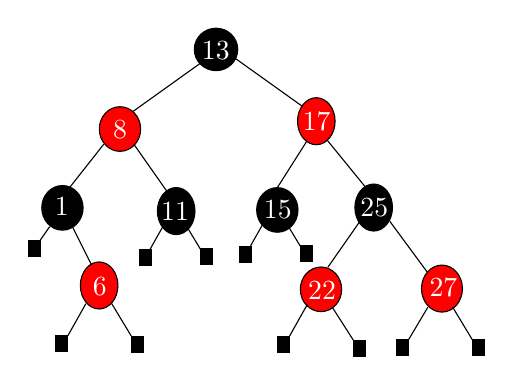
\begin{tikzpicture}[x=0.32pt,y=0.32pt,yscale=-1,xscale=1]
%uncomment if require: \path (0,706); %set diagram left start at 0, and has height of 706

\draw  [fill={rgb, 255:red, 255; green, 0; blue, 0 }  ,fill opacity=1 ]  (222.83, 160.82) circle [x radius= 23.33, y radius= 25.18]  ;
\draw  [fill={rgb, 255:red, 0; green, 0; blue, 0 }  ,fill opacity=1 ]  (150.5, 394.48) rectangle (163.83, 412.44)   ;
\draw    (163.83,394.48) -- (184.26,358.13) ;


\draw  [fill={rgb, 255:red, 0; green, 0; blue, 0 }  ,fill opacity=1 ]  (235.78, 394.91) rectangle (249.11, 412.87)   ;
\draw    (213.5,358) -- (235.78,394.91) ;


\draw  [fill={rgb, 255:red, 0; green, 0; blue, 0 }  ,fill opacity=1 ]  (286.3, 253.47) circle [x radius= 21.2, y radius= 26.53]  ;
\draw  [fill={rgb, 255:red, 0; green, 0; blue, 0 }  ,fill opacity=1 ]  (119.22, 286.65) rectangle (132.54, 304.61)   ;
\draw    (132.54,286.65) -- (143.5,271) ;


\draw  [fill={rgb, 255:red, 0; green, 0; blue, 0 }  ,fill opacity=1 ]  (331.29, 70.93) circle [x radius= 24.51, y radius= 23.93]  ;
\draw    (237.5,141) -- (314.99,85.55) ;


\draw    (238.5,178) -- (278.5,235) ;


\draw  [fill={rgb, 255:red, 0; green, 0; blue, 0 }  ,fill opacity=1 ]  (157.83, 249.82) circle [x radius= 23.33, y radius= 25.18]  ;
\draw    (163.5,230) -- (204.5,178) ;


\draw  [fill={rgb, 255:red, 255; green, 0; blue, 0 }  ,fill opacity=1 ]  (199.3, 337.47) circle [x radius= 21.2, y radius= 26.53]  ;
\draw    (169.5,272) -- (190.5,314) ;


\draw  [fill={rgb, 255:red, 255; green, 0; blue, 0 }  ,fill opacity=1 ]  (444.5, 152) circle [x radius= 21.2, y radius= 26.53]  ;
\draw    (351.5,80) -- (428.5,135) ;


\draw  [fill={rgb, 255:red, 0; green, 0; blue, 0 }  ,fill opacity=1 ]  (400.5, 252.18) circle [x radius= 23.33, y radius= 25.18]  ;
\draw    (400.5,227) -- (433.5,175) ;


\draw  [fill={rgb, 255:red, 0; green, 0; blue, 0 }  ,fill opacity=1 ]  (509.3, 249.47) circle [x radius= 21.2, y radius= 26.53]  ;
\draw    (456.5,173) -- (500.5,227) ;


\draw  [fill={rgb, 255:red, 255; green, 0; blue, 0 }  ,fill opacity=1 ]  (449.83, 341.82) circle [x radius= 23.33, y radius= 25.18]  ;
\draw    (457.5,317) -- (494.5,264) ;


\draw  [fill={rgb, 255:red, 255; green, 0; blue, 0 }  ,fill opacity=1 ]  (586.4, 341) circle [x radius= 23.1, y radius= 26.53]  ;
\draw    (527.5,265) -- (569.5,322) ;


\draw  [fill={rgb, 255:red, 0; green, 0; blue, 0 }  ,fill opacity=1 ]  (400.5, 395.48) rectangle (413.83, 413.44)   ;
\draw    (413.83,395.48) -- (434.26,359.13) ;


\draw  [fill={rgb, 255:red, 0; green, 0; blue, 0 }  ,fill opacity=1 ]  (486.78, 399.91) rectangle (500.11, 417.87)   ;
\draw    (462.5,362) -- (486.78,399.91) ;


\draw  [fill={rgb, 255:red, 0; green, 0; blue, 0 }  ,fill opacity=1 ]  (535.5, 398.48) rectangle (548.83, 416.44)   ;
\draw    (548.83,398.48) -- (570.5,362) ;


\draw  [fill={rgb, 255:red, 0; green, 0; blue, 0 }  ,fill opacity=1 ]  (620.78, 398.91) rectangle (634.11, 416.87)   ;
\draw    (598.5,362) -- (620.78,398.91) ;


\draw  [fill={rgb, 255:red, 0; green, 0; blue, 0 }  ,fill opacity=1 ]  (313.46, 295.94) rectangle (326.78, 313.91)   ;
\draw    (299.5,273) -- (321.78,309.91) ;


\draw  [fill={rgb, 255:red, 0; green, 0; blue, 0 }  ,fill opacity=1 ]  (245.16, 296.5) rectangle (258.49, 314.46)   ;
\draw    (251.83,305.48) -- (272.26,269.13) ;


\draw  [fill={rgb, 255:red, 0; green, 0; blue, 0 }  ,fill opacity=1 ]  (426.46, 292.94) rectangle (439.78, 310.91)   ;
\draw    (412.5,270) -- (434.78,306.91) ;


\draw  [fill={rgb, 255:red, 0; green, 0; blue, 0 }  ,fill opacity=1 ]  (358.16, 293.5) rectangle (371.49, 311.46)   ;
\draw    (364.83,302.48) -- (385.26,266.13) ;



\draw (331,72) node [color={rgb, 255:red, 255; green, 255; blue, 255 }  ,opacity=1 ] [align=left] {13};
\draw (157,248) node [color={rgb, 255:red, 255; green, 255; blue, 255 }  ,opacity=1 ] [align=left] {1};
\draw (285,254) node [color={rgb, 255:red, 255; green, 255; blue, 255 }  ,opacity=1 ] [align=left] {11};
\draw (223,162) node [color={rgb, 255:red, 255; green, 255; blue, 255 }  ,opacity=1 ] [align=left] {8};
\draw (445,152) node [color={rgb, 255:red, 255; green, 255; blue, 255 }  ,opacity=1 ] [align=left] {17};
\draw (401,252) node [color={rgb, 255:red, 255; green, 255; blue, 255 }  ,opacity=1 ] [align=left] {15};
\draw (510,249) node [color={rgb, 255:red, 255; green, 255; blue, 255 }  ,opacity=1 ] [align=left] {25};
\draw (200,339) node [color={rgb, 255:red, 255; green, 255; blue, 255 }  ,opacity=1 ] [align=left] {6};
\draw (451,343) node [color={rgb, 255:red, 255; green, 255; blue, 255 }  ,opacity=1 ] [align=left] {22};
\draw (588,340) node [color={rgb, 255:red, 255; green, 255; blue, 255 }  ,opacity=1 ] [align=left] {27};


\end{tikzpicture}